\section{Deadlockerkennung allgemein}
\label{section:Deadlockerkennung allgemein}
Im Gegensatz zu Single-Threaded-Anwendungen sind Multi-Threaded-Anwendungen
nicht deterministisch. Dies kann zu \emph{race conditions} führen. Eine
\emph{race condition} tritt zum Beispiel dann auf, wenn zwei Threads einen
Zähler jeweils um eins erhöhen wollen\footnote{Vgl. "Data races" in
\autocite[70]{netzer1992race}}.

Angenommen der Zähler hat zu Beginn den Wert drei. Beide Threads wollen jetzt
nahezu gleichzeitig den Zähler um eins erhöhen. Dazu lesen beide Threads den
aktuellen Wert des Zählers, in diesem Fall drei, aus. Anschließend addieren
beide eins hinzu und schreiben den neuen Wert, in diesem Fall vier, in den
Zähler. Erwartet wurde jedoch der Wert fünf, da beide Threads den Zähler um
jeweils eins erhöhen sollten. Um solche \emph{race conditions} zu verhindert
werden Synchronisationsmechanismen benötigt.

Eine Möglichkeit um den Zugriff auf eine gemeinsame Ressource zu synchronisieren
sind Locks. Ein Lock ist ein exklusiver Zugriff auf ein Objekt, ein sogenanntes
Lockobjekt. Das bedeutet, dass während ein Thread einen Lock auf ein Objekt
besitzt, andere Threads, welche auf dasselbe Objekt zugreifen wollen, warten
müssen bis es freigegeben wurde.

Betrachtet man das Beispiel mit dem Zähler erneut, dieses Mal mit Locks als
Synchronisationsmittel, kann es zu folgender Ausführung kommen. Der Zähler hat
zu Beginn wieder den Wert drei. Die Threads \textrm{T1} und \textrm{T2} wollen
erneut den Zähler nahezu gleichzeitig erhöhen. Dieses Mal versuchen beide das
Lockobjekt \textrm{L1} in Besitz zu nehmen. Der Thread \textrm{T2} nimmt
\textrm{L1} zuerst in Besitz, daraus folgt \textrm{T1} muss warten. \textrm{T2}
liest den aktuellen Wert des Zählers aus, erhöht diesen um eins und schreibt den
neuen Wert vier in den Zähler. Anschließend gibt \textrm{T2} das Lockobjekt
\textrm{L1} frei. Jetzt erhält der Thread \textrm{T1} den Zugriff auf
\textrm{L1} und liest ebenfalls den Zähler, jetzt vier, aus, erhöht diesen und
schreibt den neuen Wert fünf in den Zähler. Anschließend gibt \textrm{T1} das
Lockobjekt \textrm{L1} frei. Jetzt steht der erwartete Wert fünf im Zähler.
Durch das Lockobjekt ist die Ausführung weiterhin nicht deterministisch, da die
Reihenfolge auch erst \textrm{T1} und dann \textrm{T2} sein kann. Trotzdem ist
die korrekte Erhöhung des Zählers sichergestellt.

Die Verwendung von Locks kann in Verbindung mit der nicht deterministischen
Ausführung von Multi-Threaded-Anwendungen zu Problemen führen.

Angenommen es existieren zwei Threads \textrm{T1} und \textrm{T2} und zwei
Lockobjekte \textrm{L1} und \textrm{L2}. Angenommen \textrm{T1} besitzt
\textrm{L1} und zu gleichen Zeit erlangt \textrm{T2} das Lockobjekt \textrm{L2}.
Wenn jetzt der Thread \textrm{T1} das Lockobjekt \textrm{L2} anfordert und der
Thread \textrm{T2} das Lockobjekt \textrm{L1}, kommt es zu einem
Deadlock.\autocite[vgl.][70]{coffman1971system} Die Ausführung des Programms
terminiert nicht, da beide Threads auf den jeweils anderen Thread warten und
sich gegenseitig blockieren.

Solche potenziellen Deadlocks zu erkennen ist die Aufgabe von statischen und
dynamischen Methoden zur Deadlockerkennung. Bei der statischen Deadlockerkennung
wird der Quellcode direkt analysiert. Dieses Verfahren wird hier nicht näher
betrachtet.

Bei der dynamischen Deadlockerkennung wird die Anwendung zur Laufzeit analysiert
und läuft in folgenden drei Schritten
ab:\autocite[vgl.][212-213]{bensalem2005dynamic}
\begin{enumerate}
  \item Erstellung eines \emph{execution traces}
  \item Erstellung eines Graphen basierend auf den Informationen aus dem \emph{execution trace}
  \item Suche nach potenziellen Deadlocks durch die Identifizierung von Zyklen
  innerhalb des Graphen
\end{enumerate}
Ein \emph{execution trace} ist eine Abfolge von Events. Ein Event \textrm{$e_i$}
wird durch eine der folgenden Methoden definiert: starten eines Threads,
betreten eines Threads, Inbesitznahme eines Lockobjekts und Freigabe eines
Lockobjekts.\autocite[vgl.][212]{bensalem2005dynamic}

Die Positionsangabe der Events durch Zeilennummer wird hier ignoriert, da sie
nicht benötigt wird.\footnote{Vgl. "line number lno" in
\autocite[212]{bensalem2005dynamic}}

Das Starten eines neues Threads ist definiert durch ein Thread-Start-Event:
\begin{quote}
\texttt{s(ausführender Thread, Name des neuen Threads)}\autocite[vgl.][212]{bensalem2005dynamic}
\end{quote}
Zum Beispiel bedeutet \texttt{s(main,T1)}, dass der Thread \textrm{main} den
Thread \textrm{T1} gestartet hat. Das Betreten eines Threads ist definiert durch
ein Thread-Join-Event:
\begin{quote}
\texttt{j(ausführender Thread, Name des zu betretenden Threads)}\autocite[vgl.][212]{bensalem2005dynamic}
\end{quote}
Zum Beispiel bedeutet \texttt{j(T1,T2)}, dass der Thread \textrm{T1} den Thread
\textrm{T2} betreten hat. Die Inbesitznahme eines Lockobjekts kann definiert
werden durch ein Lock-Event:
\begin{quote}
\texttt{l(ausführender Thread, Name des Lockobjekts)}\autocite[vgl.][212]{bensalem2005dynamic}
\end{quote}
Zum Beispiel bedeutet \texttt{l(T1,L3)}, dass der Thread \textrm{T1} das
Lockobjekt \textrm{L3} in Besitz genommen hat. Die Freigabe eines Lockobjekts
kann definiert werden durch ein Unlock-Event:
\begin{quote}
\texttt{u(ausführender Thread, Name des Lockobjekts)}\autocite[vgl.][212]{bensalem2005dynamic}
\end{quote}
Zum Beispiel bedeutet \texttt{u(T1,L3)}, dass der Thread \textrm{T1} das
Lockobjekt \textrm{L3} freigegeben hat.

Die Abfolge aller während der Laufzeit des Programms aufgetretenen Events
definieren einen möglichen \emph{execution trace} des Programms. Programme
welche mit mehreren Threads arbeiten, liefern keine deterministische Abfolge.
Jede Ausführung eines solchen Programms kann zu unterschiedlichen
\emph{execution traces} führen. 

Im zweiten Schritt wird aus dem vorher erzeugten \emph{execution trace} ein
Lockgraph erstellt.

\begin{samepage}
  Ein Lockgraph ist definiert durch:
  \begin{quote}
  \textrm{LG = (L,R)}
  \end{quote}
\end{samepage}
\textrm{L} ist die Menge aller Lockobjekte im \emph{execution trace} und \textrm{R}
die Menge aller Lockpaare. Ein Lockpaar ist definiert durch das Tupel
\textrm{(L1, L2)} für das gilt: Es existiert ein Thread, welcher das Lockobjekt
\textrm{L1} besitzt, während er einen Lock auf \textrm{L2}
anfordert.\autocite[vgl.][72]{coffman1971system}\autocite[vgl.][213]{bensalem2005dynamic}

\section{PEARL}
\label{section:PEARL}
Die Programmiersprache PEARL wurde in den 1970er Jahren vom Institut für
Regelungstechnik der Universität Hannover entwickelt. PEARL ist eine Abkürzung
und steht für "Process and Experiment Automation Realtime Language". Die
Programmiersprache erlaubt eine komfortable, sichere und weitgehend
rechnerunabhängige Programmierung von Multitasking- und
Echtzeit-Aufgaben.\autocite{PEARLHistory} Das Deutsche Institut für Normung
standardisierte PEARL mehrmals, unteranderem 1998 in der DIN 66253-2 als
PEARL90\autocite{DIN-66253-2:1998-04} und zuletzt 2018 als
SafePEARL\autocite{DIN-66253:2018-03}. Nachfolgend werden PEARL und PEARL90
synonym verwendet.

In PEARL bezeichnet ein \textrm{TASK} eine Aufgabe und wird entweder direkt beim
Start des Programms oder durch Signale von anderen Aufgaben gestartet.
\textrm{TASKs} werden parallel und gemäß ihrer Priorität
ausgeführt.\autocite[vgl.][104]{PEARL} Um mehrere \textrm{TASKs} zu
synchronisieren gibt es zwei Möglichkeiten: \textrm{SEMA} und \textrm{BOLT}
Variablen.\autocite[vgl.][120]{PEARL}

Eine \textrm{SEMA} Variable ist ein Semaphor und dient als
Synchronisationsmittel. Sie kann als Wert nicht negative ganze Zahlen besitzen,
wobei null den Zustand "gesperrt" und positive Zahlen den Zustand "frei"
bedeuten.\autocite[vgl.][120]{PEARL} Eine \textrm{SEMA} Variable hat zu Beginn
den Wert null und den Zustand "gesperrt". Mit dem Befehl \textrm{RELEASE} wird
eine \textrm{SEMA} Variable um den Wert eins erhöht und erhält den Zustand
"frei". Mit dem \textrm{REQUEST} Befehl wird der Wert einer \textrm{SEMA}
Variablen um eins verringert. Ist der Wert einer \textrm{SEMA} Variablen null
wird der ausführende \textrm{TASK} angehalten und in eine Warteschlange
eingereiht. Sobald die Variable über den Befehl \textrm{RELEASE} wieder
freigeben wird, wird der nächste \textrm{TASK} in der Warteschlange gemäß seiner
Priorität fortgeführt.\autocite[vgl.][120-121]{PEARL} Das Zustandsdiagramm zur
\textrm{SEMA} Variable ist in \cref{fig:SEMA_StateDiagram} dargestellt.
\begin{figure}[ht]
  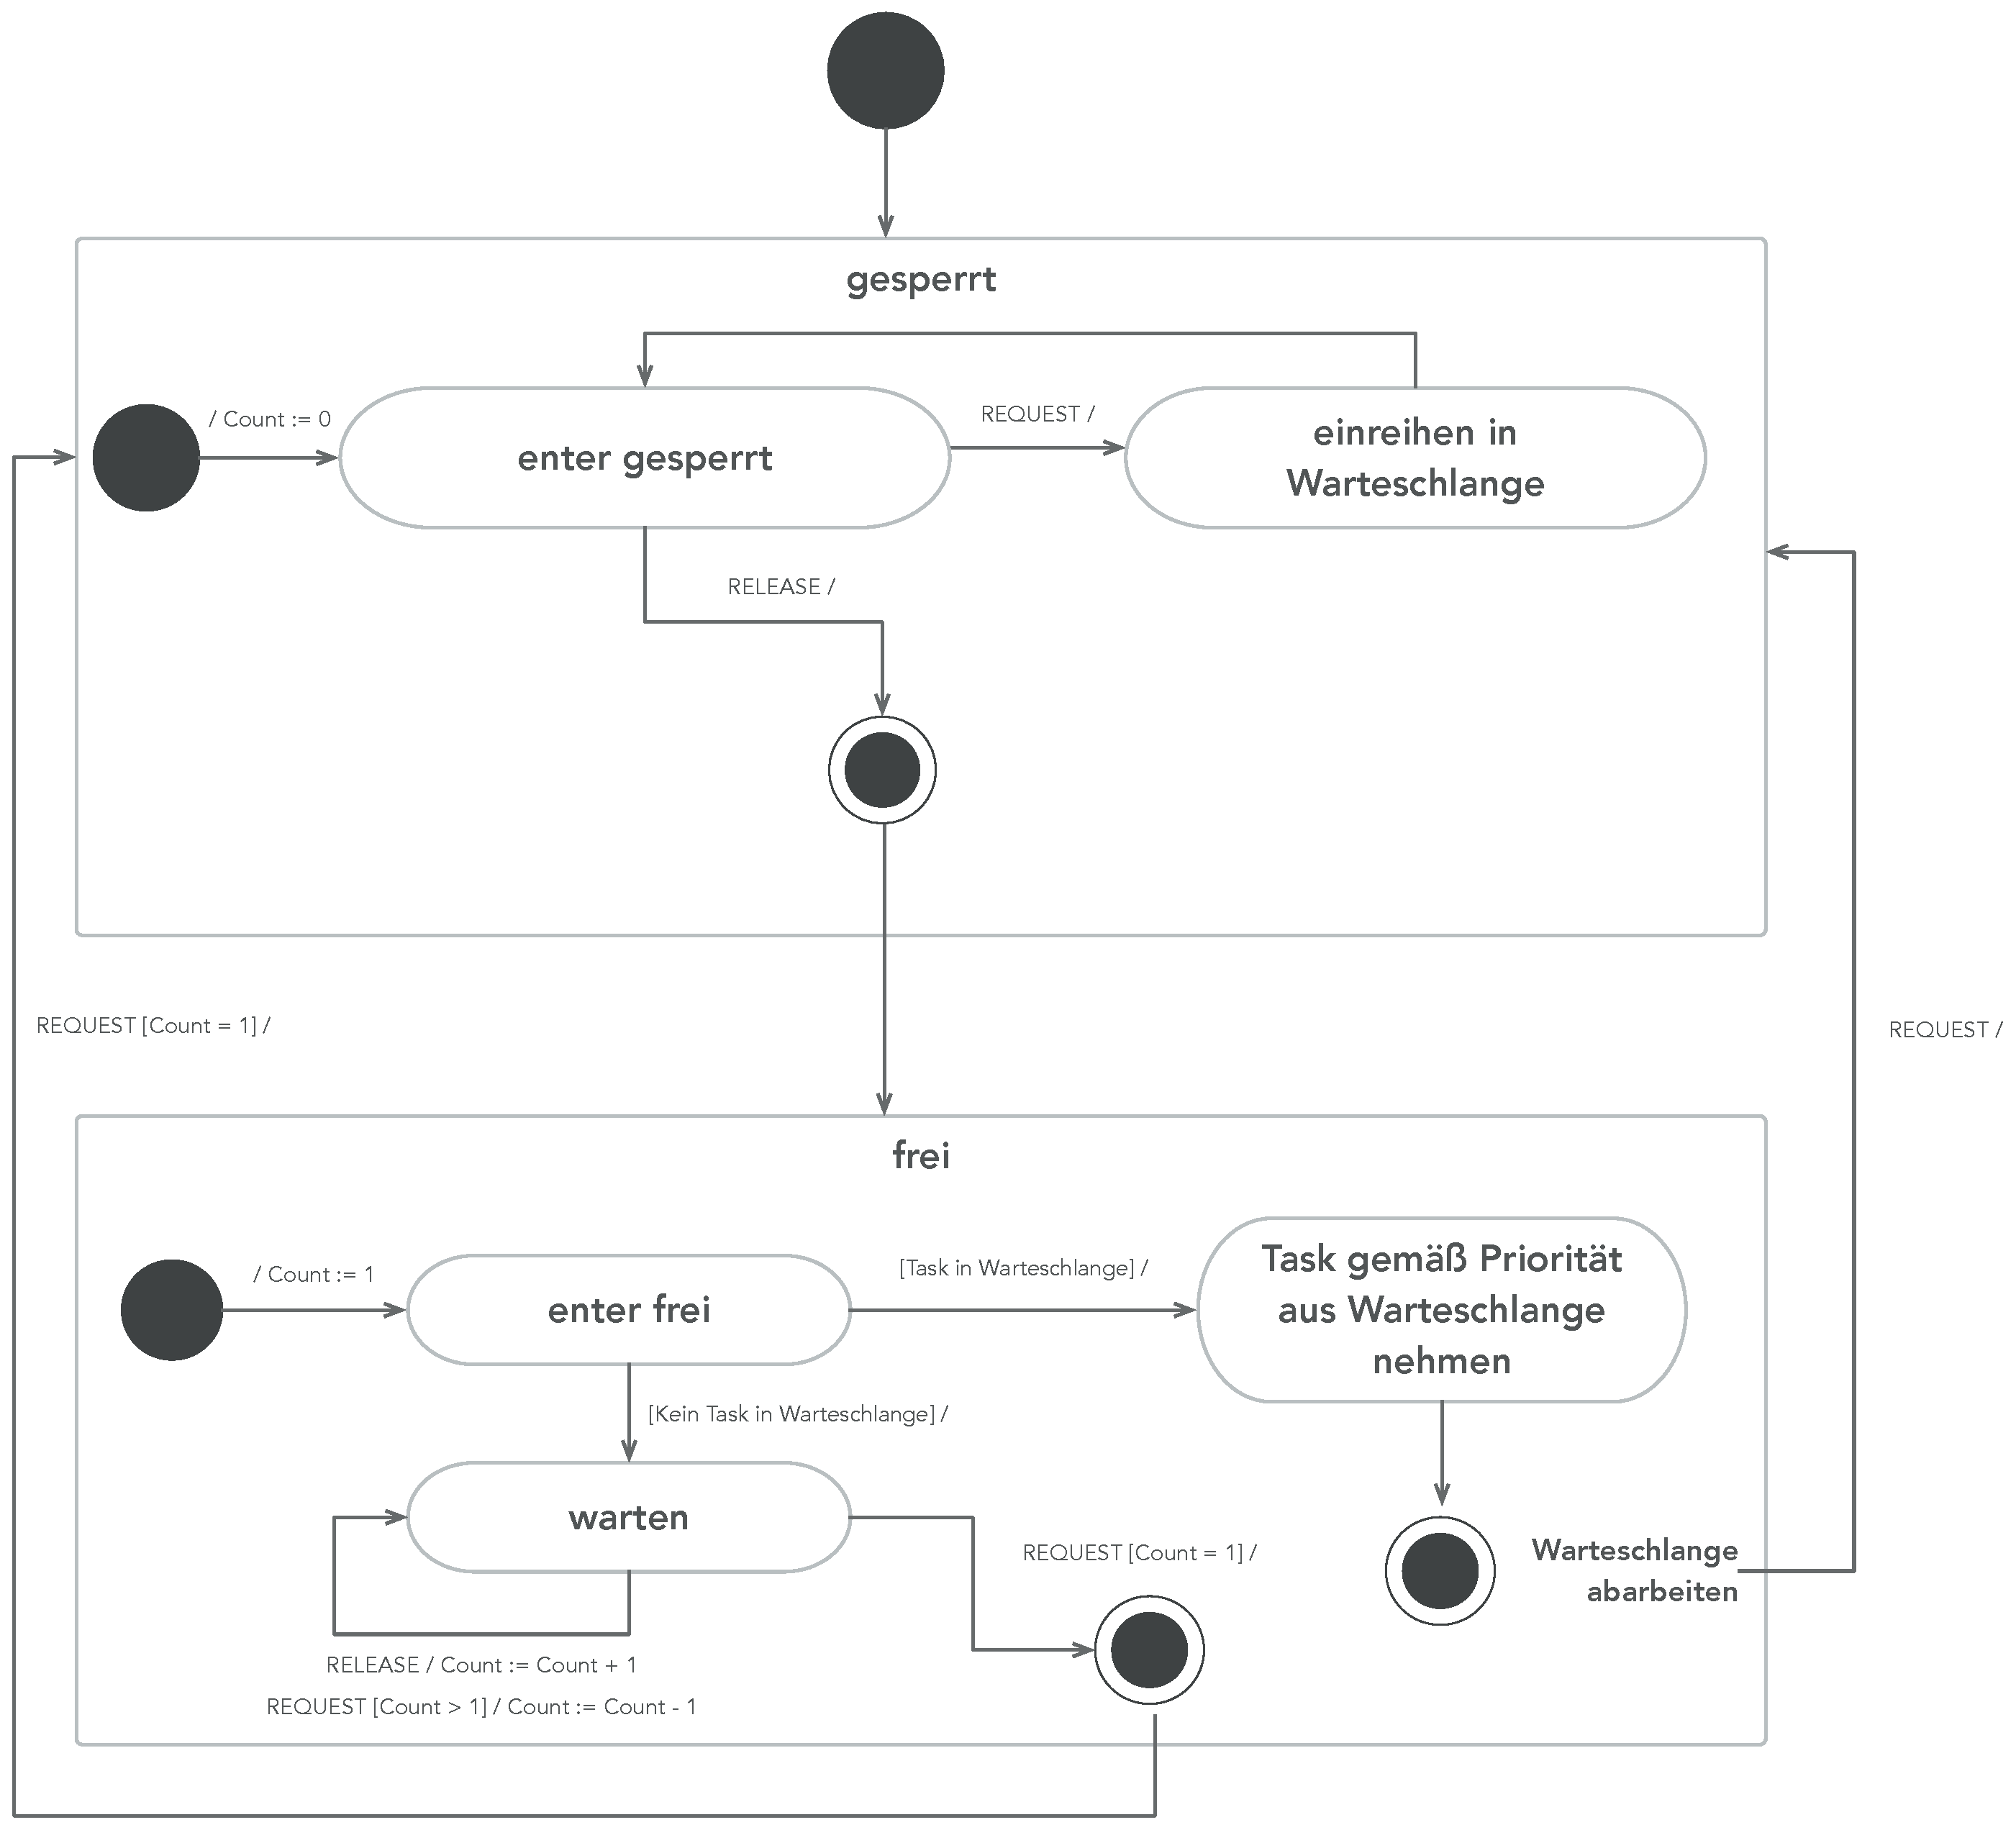
\includegraphics[width=\linewidth]{SEMA_State_Diagram.eps}
  \footnotesize\sffamily Quelle: Eigene Darstellung
  \caption{Zustandsdiagramm einer SEMA-Variablen}
  \label{fig:SEMA_StateDiagram}
\end{figure}

\textrm{BOLT} Variablen haben im Gegensatz zu \textrm{SEMA} Variablen drei
Zustände: "gesperrt", "Sperre möglich" und "Sperre nicht
möglich".\autocite[vgl.][125]{PEARL} Sie bieten die Möglichkeit exklusive und
nicht exklusive Sperren zu ermöglichen. Zum Beispiel können so simultane
Lesezugriffe und exklusive Schreibzugriffe realisiert werden. Zu Beginn hat eine
\textrm{BOLT} Variable den Zustand "Sperre möglich". Mit dem Befehl \textrm{RESERVE}
wird ein exklusiver Zugriff auf eine \textrm{BOLT} Variable angefordert. Wenn
die Variable im Zustand "Sperre möglich" ist, erhält diese den Zustand
"gesperrt". Ansonsten wird ähnlich zu der \textrm{REQUEST} Anweisung für
\textrm{SEMA} Variablen der ausführende \textrm{TASK} angehalten und in eine
Warteschlange eingereiht. Mit dem Befehl \textrm{FREE} erhält eine \textrm{BOLT}
Variable den Zustand "Sperre möglich" und alle\textrm{TASKs} in der
Warteschlange, welche aufgrund einer \textrm{RESERVE} Anweisung warten, werden
gemäß ihrer Priorität fortgeführt. Wenn keine \textrm{TASKs} in der
Warteschlange vorhanden sind, welche auf eine \textrm{RESERVE} Anweisung warten,
werden die \textrm{TASKs} in der Warteschlange gemäß ihrer Priorität
fortgeführt, welche aufgrund einer \textrm{ENTER} Anweisung warten. Mit der
\textrm{ENTER} Anweisung wird ein nicht exklusiver Zugriff angefordert. Wenn die
\textrm{BOLT} Variable im Zustand "gesperrt" ist oder ein \textrm{TASK} in der
Warteschlange existiert, welcher einen exklusiven Zugriff mittels einer
\textrm{RESERVE} Anweisung angefordert hat, wird der ausführende \textrm{TASK}
angehalten und in eine Warteschlange eingereiht. Ansonsten erhält die Variable
den Zustand "Sperre nicht möglich", um den exklusiven Zugriff zu verbieten.
Zusätzlich wird die Anzahl der benutzenden \textrm{TASKs} um eins erhöht. Die
\textrm{LEAVE} Anweisung verringert die Anzahl der benutzenden \textrm{TASKs} um
eins, wenn die Anzahl eins entspricht, funktioniert die
\textrm{LEAVE} Anweisung wie die \textrm{FREE}
Anweisung.\autocite[vgl.][125-127]{PEARL} Das Zustandsdiagramm zur \textrm{BOLT}
Variable ist in \cref{fig:BOLT_StateDiagram} dargestellt.
\begin{figure}[ht]
  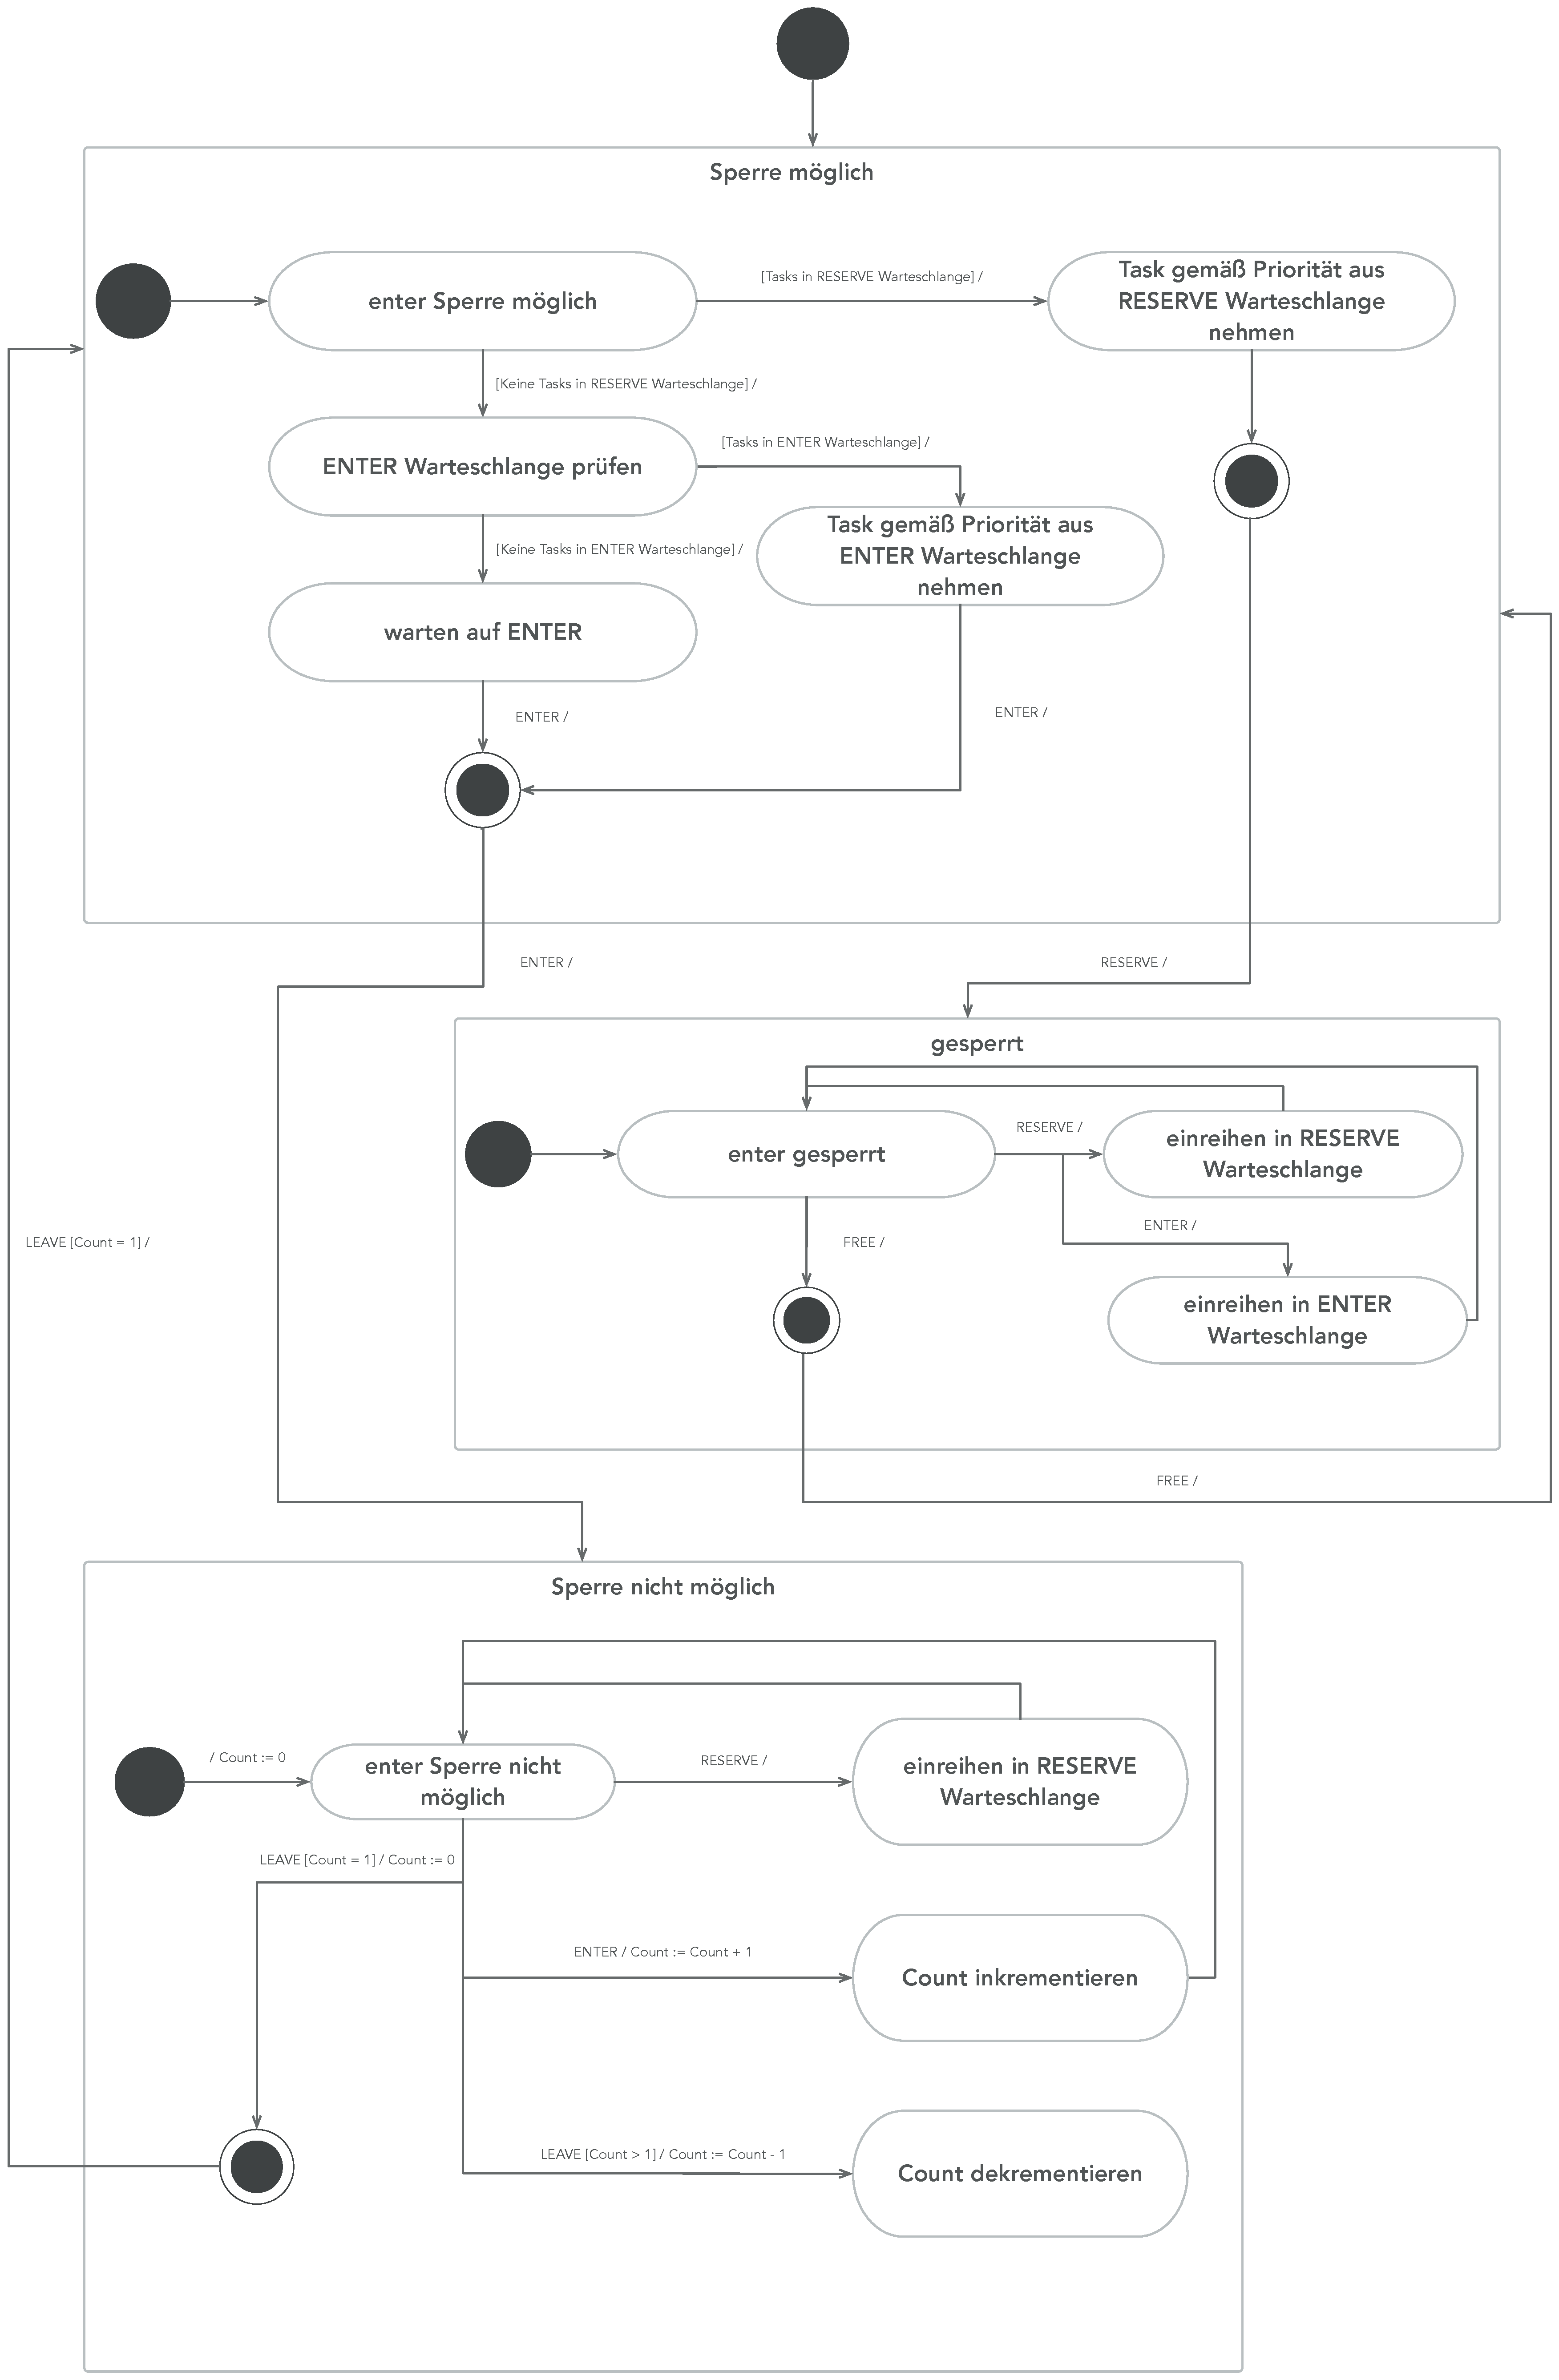
\includegraphics[width=\linewidth]{BOLT_State_Diagram.eps}
  \footnotesize\sffamily Quelle: Eigene Darstellung
  \caption{Zustandsdiagramm einer BOLT-Variablen}
  \label{fig:BOLT_StateDiagram}
\end{figure}

\section{OpenPEARL}
\label{section:OpenPEARL}
Um PEARL Programme auf einem System auszuführen wird ein Compiler benötigt. Das
OpenSource Projekt OpenPEARL besteht aus einem Compiler und einer
Laufzeitumgebung für PEARL.\autocite{OpenPEARL_Structure} Unterstützt wird der
PEARL90 Standard bis auf einige wenige
Unterschiede.\autocite{OpenPEARL_Differences_To_PEARL90}

OpenPEARL besteht aus drei wesentlichen
Komponenten:\autocite{OpenPEARL_Structure}
\begin{enumerate}
  \item Compiler
  \item Laufzeitumgebung
  \item Inter Module Checker
\end{enumerate}
Der Compiler ist in Java geschrieben und übersetzt PEARL Code in C++ Code. Die
Laufzeitumgebung stellt dem Compiler eine API zur Verfügung. Dem Compiler werden
durch die API sichere Implementierungen der PEARL Datentypen zur Verfügung
gestellt. Zusätzlich enthält die Laufzeitumgebung plattformspezifische Anteile
für zum Beispiel die Implementierung für das Scheduling der Tasks. PEARL
Anwendungen können aus mehreren Modulen bestehen, welche unabhängig voneinander
kompiliert werden. Um Inkonsistenzen bei der Erstellung der Anwendung zu
verhindern, prüft der Inter Module Checker die Export- und Importschnittstellen
aller Module und deren Kompatibilität.\autocite{OpenPEARL_Structure}

In \cref{lst:ExampleDeadlock} ist ein Beispielprogramm in der Programmiersprache
PEARL dargestellt. Das Programm startet zwei parallele Aufgaben welche beide
eine Zeichenfolge auf der Standardausgabe ausgeben. Der Zugriff auf die
Standardausgabe muss dabei synchronisiert erfolgen.
\begin{listing}[ht]
  \inputminted[frame=lines,linenos]{vim}{./Examples/Example_Deadlock.prl}
  \caption{Beispiel einer OpenPEARL-Anwendung mit einem potenziellen Deadlock}
  \label{lst:ExampleDeadlock}   
\end{listing} 
In den Zeilen~7 bis 10 werden Variablen definiert, wie zum Beispiel die Ausgabe
über die Standardausgabe und die zwei \textrm{SEMA} Variablen \textrm{L1} und
\textrm{L2} in den Zeilen~9 und 10. In den Zeilen~12 bis 17 ist ein \textrm{TASK}
definiert.

Durch die Kennzeichnung \textrm{MAIN} wird der \textrm{TASK} direkt beim Start
des Programms ausgeführt\autocite[vgl.][28]{PEARL}. Die Befehle \textrm{RELEASE}
in den Zeilen~13 und 14 erhöhen den Wert der jeweiligen \textrm{SEMA} Variable
um eins, wodurch der Zustand von "gesperrt" auf "frei" gesetzt wird.
Anschließend werden in den Zeilen~15 und 16 die \textrm{TASKS} \textrm{T2} und
\textrm{T3} gestartet.

Die \textrm{TASKS} \textrm{T2} und \textrm{T3} geben in den Zeilen~22 bis 24 und
in den Zeilen~32 bis 34 die Zeichenfolge "Hello World T2" bzw. "Hello World T3"
auf der Standardausgabe aus. Die Synchronisierung des Zugriffs auf die
Standardausgabe erfolgt mittels den \textrm{SEMA} Variablen \textrm{L1} und
\textrm{L2}. Beide \textrm{TASKS} versuchen beide \textrm{SEMA} Variablen in
Besitz zu nehmen. \textrm{T2} versucht in den Zeilen~20 und 21 zuerst
\textrm{L1} und dann \textrm{L2} in Besitz zu nehmen. \textrm{T3} versucht in
den Zeilen~30 und 31 zuerst \textrm{L2} und dann \textrm{L1} in Besitz zu
nehmen. Da beide \textrm{TASKS} parallel laufen, kann es passieren, dass
\textrm{T2} \textrm{L1} in Zeile~20 in Besitz nimmt und gleichzeitig \textrm{T3}
in Zeile~30 \textrm{L2} in Besitz nimmt. Beide \textrm{SEMA} Variablen haben
jetzt den Wert null und den Zustand "gesperrt". Der \textrm{TASK} \textrm{T2}
wartet jetzt darauf, dass \textrm{L2} freigegeben wird und
\textrm{T3} wartet darauf, dass \textrm{L1} freigegeben wird. Beide \textrm{TASKS}
warten auf den jeweils anderen und verursachen einen Deadlock.

\section{MagicLock}
\label{section:MagicLock}
MagicLock ist ein Algorithmus zur dynamischen Deadlockerkennung. Während der
Entwicklung wurde der Fokus auf die Skalierung und Effizienz des Algorithmus
gesetzt. Ziel war es mit großen Multithreaded Anwendungen skalieren und diese
effizient analysieren zu können.\autocite[vgl.][1]{MagicLock}

MagicLock analysiert einen \emph{execution trace} einer Programmausführung ohne
Deadlocks \autocite[vgl.][4]{MagicLock}. Ein möglicher \emph{execution trace}
von dem Beispielprogramm aus \cref{lst:ExampleDeadlock} ist:
\begin{quote}
  \textbf{$\sigma$} = s(main,T1), u(T1,L1), u(T1,L2), s(T1,T2), s(T1,T3),
  l(T2,L1), l(T2,L2), u(T2,L2), u(T2,L1), l(T3,L2), l(T3,L1), u(T3,L1), u(T3,L2)
\end{quote}
Der \emph{execution trace} in MagicLock wird durch eine Lock-Dependency-Relation
definiert. Eine Lock-Dependency-Relation \textrm{D} besteht aus einer Sequenz
von Lock-Dependencies. Eine Lock-Dependency ist ein Tripel \textrm{r = (t,m,L)}
in dem \textrm{t} ein Thread ist, \textrm{m} ein Lockobjekt und \textrm{L} eine
Menge von Lockobjekten. Das Tripel sagt aus, dass der Thread \textrm{t} das
Lockobjekt
\textrm{m} in Besitz nimmt, während er jedes Lockobjekt in \textrm{L} besitzt.\autocite[vgl.][3]{MagicLock}

Bei einem Thread-Start-Event wird ein neuer Thread-Identifier und eine leere
Menge an Locks für den neu erzeugten Thread erstellt
\autocite[vgl.][4]{MagicLock}. Zum Beispiel wird bei den Event \textrm{s(main,T1)}
ein neuer Thread-Identifier für \textrm{T1} erzeugt und eine leere Menge
\textrm{$L_T1$}.

Bei einem Lock-Event \textrm{l(T2,L1)} wird zuerst die Lock-Dependency
\textrm{$(T2,L1,L_T2)$} an den \emph{execution trace} angehängt und anschließend
\textrm{L1} in die Menge der Locks
\textrm{$L_T2$} eingefügt. Bei einem Unlock-Event \textrm{u(T2,L2)}
wird das Lockobjekt \textrm{L2} aus der Menge \textrm{$L_T2$}
entfernt.\autocite[vgl.][4]{MagicLock}

Daraus folgt die Lock-Dependency-Relation:
\begin{quote}
  \textbf{$D_\sigma$} = (T2,L1,\{\}), (T2,L2,\{L1\}), (T3,L2,\{\}),
  (T3,L1,\{L2\})
\end{quote}
Anschließend wird ein reduzierter \emph{execution trace} erzeugt. Dazu verwendet
MagicLock einen Algorithmus zur Reduzierung von Lockobjekten im \emph{execution
trace}. Der Algorithmus entfernt alle Lockobjekte aus der Menge aller
Lockobjekte \textrm{Locks} aus \textrm{$D_\sigma$} die entweder keine
eingehenden \textrm{indegree(m) = 0} oder keine ausgehenden \textrm{outdegree(m)
= 0} Kanten im Lockgraph besitzen. Die Annahme ist, dass ein Lockobjekt nur Teil
eines Zyklus sein kann, wenn dieses mindestens eine eingehende und mindestens
eine ausgehende Kante besitzt. Zusätzlich werden alle Lockobjekte entfernt,
welche nur von einem einzigen Thread in Besitz genommen bzw. freigegeben wurden.
Wenn nur ein Thread ein Lockobjekt benutzt, kann dieses Lockobjekt nicht Teil
eines Deadlocks sein. Mit den reduzierten Lockobjekten wird im nächsten Schritt
die Zyklensuche vorbereitet.\autocite[vgl.][4]{MagicLock}

Die noch vorhandenen Lock-Dependencies werden in Partitionen basierend auf ihrer
Thread ID unterteilt und anschließend sortiert. Für jeden Thread wird eine
Partition erstellt mit allen Lock-Dependencies mit \textrm{($t_i$,m,L)} wobei
\textrm{$t_i$} der jeweilige Thread der Partition ist. Zusätzlich werden gleiche
Lock-Dependencies in Gruppen eingeteilt. Für gleiche Lock-Dependencies muss dann
immer nur ein Element aus der Gruppe geprüft werden. Wenn ein Zyklus gefunden
wurde, wurde gleichzeitig ein Zyklus für alle Lock-Dependencies in der Gruppe
gefunden. Wenn kein Zyklus gefunden wurde, wird dies gleichzeitig für alle
anderen Elemente in der Gruppe angenommen.\autocite[vgl.][8-9]{MagicLock}

Zwei Lock-Dependencies sind gleich wenn folgendes
gilt:\autocite[vgl.][8]{MagicLock}
\begin{quote}
  Gegeben sind zwei Lock-Dependencies \textrm{$r_1 = (t_1, m_1, L_1)$} und
  \textrm{$r_2 = (t_2, m_2, L_2)$}: $r_1 = r_2 \Leftrightarrow t_1 = t_2 \land
  m_1 = m_2 \land L_1 = L_2 $
\end{quote}
Anschließend werden die Partitionen gegeneinander auf Lock-Dependency-Chains
geprüft \autocite[vgl.][8]{MagicLock}. Eine Lock-Dependency-Chain ist eine
Sequenz von Lock-Dependencies für die gilt:\autocite[vgl.][3]{MagicLock}
\begin{quote}
  \textbf{$d_{chain}$} = $(r_1, r_2, \dots , r_k)$ mit $r_i = (t_i, m_i, L_i)$,
  wenn $m_1 \in L_2 \dots m_{k-1} \in L_k, t_i \neq t_j$ und $L_i \cap L_j =
  \emptyset$ für $1 \leq i, j \leq k (i \neq j)$
\end{quote}
Eine Zyklische-Lock-Dependency-Chain ist eine Lock-Dependency-Chain für die
zusätzlich gilt:\autocite[vgl.][3]{MagicLock}
\begin{quote}
  $m_k \in L_1$
\end{quote}
Zum Beispiel ist die Lock-Dependency Sequenz \textrm{$d = (t_1, l_2, \{l_1\}),
(t_2, l_1, \{l_2\})$} eine Zyklische-Lock-Dependency-Chain. Jede
Zyklische-Lock-Dependency-Chain repräsentiert einen potenziellen
Deadlock\autocite[vgl.][3]{MagicLock}.